\chapter{Dasar Teori}
\label{chap:definition}
Pada bab ini akan dijelsaskan mengenai konsep-konsep dasar pengukung PL, yaitu Java FX, Apache POI, iCal4j.

\section{Apache POI}

Apache POI pada hakikatnya merupakan \textit{library} untuk memanipulasi dan menciptakan sesuatu melalui Java API( \textit{application programming interface}) dengan memanipulasi berbagai format file berdasarkan \textit{Office Open XML standards}(OOXML) dan dokumen \textit{Microsoft OLE 2 Document Compound Format}(OLE2), Singkatnya dengan library ini memungkinkan untuk membaca dan menulis pada MS Excel menggunakan Java \cite{apachepoi}. \\


\subsection{Komponen Apache POI}
Untuk membaca aplikasi MS Office Apache POI mempunyai modul berisi komponen java api untuk membaca dokumen dengan format OLE2 dan OOXML. Berikut ini komponen-komponen dalam Apache POI.\cite{apachepoi}  

\begin{enumerate}
	\item Excel \textit{workbooks} (HSSF dan XSSF)
	\item Word \textit{document} (HWPF dan XWPF)
	\item PowerPoint \textit{presentation} (HSLF dan XSLF)
	\item Outlook (HSMF)
	\item Visio (HDGF dan XDGF)
	\item Publisher (HPBF)
\end{enumerate}

HSSF dan XSSF memberikan cara untuk membuat, membaca, dan memodifikasi XLS spreadsheet. Pada sub bab ini akan di fokuskan untuk membahas HSSF dan XSSF sesuai kebutuhan untuk menganalisa file excel jadwal mengawas ujian yang dikeluarkan oleh TU FTIS.\cite{apachepoi}


\subsection{Kelas Inti Apache POI} 
Pada sub bab ini akan membahas sedikit intoduksi mengenai beberapa kelas dan method yang ada di Apache POI API yang merupakan bagian penting untuk bekerja dengan file excel mengunakan program Java.\cite{apachepoi2}

\subsubsection{Workbook}
\textbf{org.apache.poi.ss.usermodel} \textit{package} merupakan \textit{super-interface} dari semua kelas yang berhubungan dengan pembuatan atau\textit{maintain} Excel workbook. Dua kelas yang mengimplementasikan \textit{interface} diatas sebagai berikut:\cite{apachepoi2}

\begin{itemize}
	\item \textbf{HSSFWorkbook} : Kelas ini mempunyai method yang dapat membaca dan menulis file Microsoft Excel dengan format .xls. Kelas ini kompatibel dengan MS-Office versi 97-2003.
	\item \textbf{XSSFWorkbook} : Kelas ini mempunyai method untuk menulis dan membaca Microsoft Excel dan OpenOffice xml dengan format .xls atau .xlsx. Kelas ini kompatibel dengan MS-Office versi 2007 atau versi barunya.
\end{itemize}  


\subsubsection{HSSFWorkbook} 
HSSFWorkbook merupakan \textit{high-level class} dibawah \textbf{org.apache.hssf.usermodel} \textit{package}. HSSFWorkbook juga mengimplementasikan antarmuka workbook yang digunakan oleh file Excel dalam format .xls. Berikut ini list dari bebeberapa method dan constructor dalam kelas ini.\cite{apachepoi2}\\

\noindent \textbf{Class Constructor}\\ \\


	\begin{tabular}{|c|p{12cm}|}
		\hline
		\textbf{No} & \textbf{Constructor dan Deskripsi} \\ \hline \hline
		1 & \textbf{HSSFWorkbook()}\\
			&	Membuat baru objek HSSFWorkbook.\\ \hline 
		2 & \textbf{HSSFWorkbook(DirectoryNode directory, boolean perserveNodes)}\\
			&	Membuat objek HSSFWorkbook baru dalam direktori yang spesifik.\\ \hline
		3 & \textbf{HSSFWorkbook(DirectoryNode directory, POIFSFileSystem fs, boolean perserveNodes)}\\
			&	Memberikan sebuah objek POIDSFileSystem dan sebuah spesifik didalamnya, serta membuat objek SSFWorkbook untuk membaca sebuah workbook yang spesifik.\\ \hline 
		4 & \textbf{HSSFWorkbook(java.io.InputStream s)}\\
			&	Membuat baru objek HSSFWorkbook menggunakan input stream.\\ \hline
		5 & \textbf{HSSFWorkbook(java.io.InputStream s, boolean preserveNodes )}\\
			&	Membangun sebuah POI \textit{file system} disekeliling input stream.\\ \hline
		6 & \textbf{HSSFWorkbook(POIFSFileSystem fs)}\\
			&	Membangun sebuah objek HSSFWorkbook baru menggunakan sebuah objek POIFSFileSystem.\\ \hline 		
		7 & \textbf{HSSFWorkbook(POIFSFileSystem fs, boolean preserveNodes)}\\
			&	Memberikan sebuah objek POIFSFileSystem dan membuat HSSFWorkbook baru untuk membacu sebuah workbook spesifik.\\ \hline 
	\end{tabular}

Berikut ini penjelasan parameter yang sering dipakai pada constructor :
\begin{itemize}
	\item \textbf{directory} : direktori proses dari POI filesystem
	\item \textbf{fs} : POI filesystem yang mengandung workbook stream.
	\item \textbf{preservenodes} : Opsional parameter yang memutuskan menjaga node lain, selain itu parameter ini menggunakan banyak memori seperti menyimpan semua POIFileSystem dalam memori(jika diset).
\end{itemize} 

\subsubsection{XSSFWorkbook}
Kelas ini merepresentasikan baik \textit{high} dan \textit{low} level format file excel. XSSFWorkbook merupakan kelas yang berada dalam \textit{package} \textbf{org.apache.xssf.usermodel} dan mengimplementasikan antarmuka workbook. Berikut ini list method dan constructor dalam kelas ini.\cite{apachepoi2}
\\
\noindent \textbf{Class Constructor}\\ \\
	\begin{tabular}{|c|p{12cm}|}
		\hline
		\textbf{No} & \textbf{Constructor dan Deskripsi} \\ \hline \hline
		1 & \textbf{XSSFWorkbook()}\\
			&	Membuat baru objek XSSFWorkbook.\\ \hline 
		2 & \textbf{XSSFWorkbook(java.io.File file)}\\
			&	Membangun sebuah objek XSSFWorkbook dari file yang diberikan.\\ \hline
		3 & \textbf{XSSFWorkbook(java.io.InputStream is)}\\
			&	Membangun sebuah object XSSFWorkbook dengan \textit{buffering} semua input stream kedalam memory, dilanjutkan dengan membuka objek OPCPackage.\\ \hline 
		4 & \textbf{XSSFWorkbook(java.lang.String path)}\\
			&	Membangun sebuah objek XSSFWorkbook dengan diberikan \textit{full path} dari sebuah file.\\ \hline
	\end{tabular}
\\
\noindent \textbf{Class Methods}\\ \\

	\begin{tabular}{|c|p{12cm}|}
		\hline
		\textbf{No} & \textbf{Method dan Deskripsi} \\ \hline \hline
		1 & \textbf{CreateSheet()}\\
			&	Menciptakan sebuah XSSFSheet pada workbook, lalu menambahkan sheet, dan mengembalikannya dalam representasi \textit{high level} .\\ \hline 
		2 & \textbf{createSheet(java.lang.String sheetname)}\\
			&	Membuat sheet baru untuk workbook dan mengembalikannya dalam representasi \textit{high level}.\\ \hline
		3 & \textbf{createFont()}\\
			&	Membuat font baru dan menambahkannya pada tabel font workbook.\\ \hline 
		4 & \textbf{createCellStyle()}\\
			&	Membuat XSSFCellStyle Baru dan mmenambahkannya pada tabel style workbook.\\ \hline
		5 & \textbf{setPrintArea(int sheetIndex, int startColumn, int endColumn, int startRow,int endRow)}\\
			&	Menentukan area print dari kertas yang diberikan dengan parameter yang spesifik.\\ \hline	
	\end{tabular}
	
	
\subsubsection{Sheet}
Sheet merupakan sebuah interface dibawah package org.apache.ss.usermodel dan sheet merupakan super-interface dari semua kelas yang menciptakan \textit{high} atau \textit{low level spreadsheet} dengan nama yang spesifik. Jenis yang paling umum dari spreadsheet adalah worksheet yang direpresentasikan sebagai sebuah \textit{grid} dari cell.\cite{apachepoi2}

\subsubsection{HSSFSheet}
HSSFSheet merupakan kelas dibawah \textit{package}\textbf{org.apache.poi.hssf.usermodel}. HSSFSheet dapat membuat excel spreadsheet dan memungkinkan untuk memformat style dari sheet dan data sheet.\cite{apachepoi2}
\\
\noindent \textbf{Class Constructor}\\ \\
	\begin{tabular}{|c|p{12cm}|}
		\hline
		\textbf{No} & \textbf{Constructor dan Deskripsi} \\ \hline \hline
		1 & \textbf{HSSFSheet(HSSFWorkbook workbook)}\\
			&	Membuat baru HSSFSheet yang disebut HSSFWorkbook dalam pembuatan sheet baru .\\ \hline 
		2 & \textbf{HSSFSheet(HSSFWorkbook workbook, InternalSheet sheet)}\\
			&	Membuat sebuah HSSFSheet yang mewakili objek sheet yang diberikan.\\ \hline
	\end{tabular}
	
\subsubsection{XSSFSheet}
Kelas ini merupakan representasi dari \textit{high level} excel spreadsheet. Kelas ini berada dibawah package org.apache.poi.hssf.usermodel.\cite{apachepoi2}
\\
\noindent \textbf{Class Constructor}\\ \\
	\begin{tabular}{|c|p{12cm}|}
		\hline
		\textbf{No} & \textbf{Constructor dan Deskripsi} \\ \hline \hline
		1 & \textbf{XSSFSheet()}\\
			&	Membuat baru XSSFSheet yang disebut XSSFWorkbook dalam pembuatan sheet baru .\\ \hline 
		2 & \textbf{XSSFSheet(PackagePart part, PackageRelationship rel)}\\
			&	Membuat sebuah XSSFSheet yang mewakili bagian package dan \textit{relationship}.\\ \hline
	\end{tabular}
\\
\noindent \textbf{Class Method}\\ \\
	\begin{tabular}{|c|p{12cm}|}
		\hline
		\textbf{No} & \textbf{Constructor dan Deskripsi} \\ \hline \hline
		1 & \textbf{addMergedRegion(CellRangeAddress region))}\\
			&	Menambahkan gabungan wilayah dari cell.(beberapa cell menjadi satu)   .\\ \hline 
		2 & \textbf{autoSizeColumn(int column)}\\
			& Menyesuaikan lebar kolom agar sesuai dengan isinya.\\ \hline
		3 & \textbf{iterator()}\\
			&	Method ini alias rowIterator() untuk memungkinkan foreach loop .\\ \hline
		4 & \textbf{addHyperlink(XSSFHyperlink hyperlink)}\\
			&	Mendaftarkan sebuah hyperlink kedalam koleksi hyperlink yang ada di sheet.\\ \hline	
	\end{tabular}

\subsubsection{Row}
Row merupakan interface berada dibawah \textit{package} \textbf{org.apache.poi.ss.usermodel}. Row ini digunakan untuk \textit{high-level representation} dari sebuah row pada sebuah spreadsheet. Row juga merupakan super-interface dari semua kelas yang mewakili row dalam POI \textit{Library}.\cite{apachepoi2}

\subsubsection{XSSFRow}
XSSFRow merupakan sebuah kelas dibawah \textit{package} \textbf{org.apache.poi.xssf.usermodel} dan mengimplementasi Row interface. Selain itu, kelas ini dapat membuat row dalam sebuah spreadsheet. List dibawah ini merupakan method dan constructors pada kelas ini.\cite{apachepoi2}
 \\ 
\noindent \textbf{Class Method}\\ \\
	\begin{tabular}{|c|p{12cm}|}
		\hline
		\textbf{No} & \textbf{Deskripsi} \\ \hline \hline
		1 & \textbf{createCell(int columnIndex)}\\
			&	Membuat cell baru dalam baris.\\ \hline 
		2 & \textbf{setHeight(short height)}\\
			&	Mengatur tinggi dalam satuan short.\\ \hline
	\end{tabular}

\subsubsection{Cell}
Cell merupakan interface yang berada dibawah \textit{package} \textbf{org.apache.poi.ss.usermodel}. Cell merupakan sebuah super-interface dari semua kelas yang mewakili cell dalam baris sebuah spreadsheet.\\

Cell dapat beruba berbagai atrubut seperti \textit{blank, numeric, date, error, } dll. Sebelum ditambahkan ke baris cell memiliki nomer tersendiri(dari mulai 0).\cite{tutpoint}

\subsubsection{XSSFCell}  
Kelas ini berada dibawah \textit{package} \textbf{org.apache.poi.xssf.usermodel}. Kelas ini mewakili cell interface. XSSFCell adalah \textit{high-level representation} cell dalam row dari sebuah spreadsheet.\cite{tutpoint}

\subsubsection{Ringkasan Tipe Cell}
List dibawah ini adalah sebagian \textit{field} dari kelas XSSFCell beserta deskripsinya.\\

	\begin{tabular}{|c|c|}
		\hline
		\textbf{Tipe Cell} & \textbf{Deskripsi} \\ \hline \hline
		CELL\_TYPE\_BLANK & Representasi cell kosong\\ \hline 
		CELL\_TYPE\_BOOLEAN &	Representasi cell Boolean (True atau False)\\ \hline 
		CELL\_TYPE\_ERROR & Representasi nilai error dari cell\\ \hline
		CELL\_TYPE\_FORMULA	&	Representasi dari hasil sebuah formula dalam cell\\ \hline
		CELL\_TYPE\_NUMERIC	&	Representasi dari data numerik dalam cell\\ \hline
		CELL\_TYPE\_STRING	&	Representasi dari String(teks) dalam cell\\ \hline
	\end{tabular}
	\\
	
\noindent \textbf{Class Method}\\ \\
	\begin{tabular}{|c|p{12cm}|}
		\hline
		\textbf{No} & \textbf{Deskripsi} \\ \hline \hline
		1 & \textbf{setCellStyle(CellStyle style)}\\
			&	Mengatur style untuk cell.\\ \hline 
		2 & \textbf{setCellType(int cellType)}\\
			&	Mengatur tipe cell (numeric, formula, atau String).\\ \hline
		3 & \textbf{setCellValue(boolean value)}\\
			&	Mengatur nilai bolean dalam sebuah cell.\\ \hline
		4 & \textbf{setCellValue(java.util.Calendar value)}\\
			&	Mengatur nilai tanggal dari cell .\\ \hline	
		5 & \textbf{setCellValue(double value)}\\
			&	Mengatur nilai numerik dari cell.\\ \hline
		6 & \textbf{setCellValue(java.lang.String str)}\\
			&	Mengatur nilai String dari cell.\\ \hline
		7 & \textbf{setHyperlink(Hyperlink hyperlink)}\\
			&	Menambahkan sebuah hyperlink kedalam cell\\ \hline					
	\end{tabular}

\subsubsection{XSSFCellStyle}
XSSFCellStyle merupakan sebuah kelas yang berada dibawah \textit{package} \textbf{org.apache.poi.usermodel}. kelas ini memberikan infomarsi yang mungkin mengenai format konten pada suatu cell dari spreadsheet. Kelas ini juga memberikan opsi untuk merubah format tersebut. Kelas ini mewakili CellStyle interface.\cite{apachepoi2}

\subsubsection{Ringkasan Cell Style}
List dibawah ini adalah sebagian \textit{field} yang diwariskan dari CellStyle interface.\cite{tutpoint}\\

	\begin{tabular}{|c|c|}
		\hline
		\textbf{Nama Field} & \textbf{Deskripsi Field} \\ \hline \hline
		ALIGN\_CENTER & Rata tengah konten cell\\ \hline 
		ALIGN\_CENTER\_SELECTION &	Posisi seleksi tengah horizontal\\ \hline 
		ALIGN\_FILL & Mencocokan ukuran konten cell \\ \hline
		ALIGN\_JUSTIFY	&	Mencocokan ukuran konten cell terhadap lebarnya\\ \hline
		ALIGN\_LEFT	&	Rata kiri konten cell\\ \hline
		ALIGN\_RIGHT &	Rata kanan konten cell\\ \hline
		BORDER\_DASH\_DOT &	Cell style dengan garis dan titik \\ \hline
		BORDER\_DOTTED &	Cell style dengan border titik\\ \hline
		BORDER\_DASHED &	Cell Style dengan border garis\\ \hline
		BORDER\_THICK &	Cell Style dengan border tebal\\ \hline
		BORDER\_THIN &	Cell Style dengan border tipis\\ \hline
		VERTICAL\_BOTTOM &	Posisi konten cell vertikal kebawah\\ \hline
		VERTICAL\_CENTER &	Posisi konten cell vertikal ketengah\\ \hline
		VERTICAL\_JUSTIFY &	Posisi konten cell sejajar secara vertikal \\ \hline
		VERTICAL\_TOP &	Posisi selaras keatas secara vertikal\\ \hline
	\end{tabular}
\\
\noindent \textbf{Class Constructor}\\ \\
	\begin{tabular}{|c|p{15cm}|}
		\hline
		\textbf{No} & \textbf{Constructor dan Deskripsi} \\ \hline \hline
		1 & \textbf{XSSFCellStyle(int cellXfId, int cellStyleXfId, StylesTable stylesSource, ThemesTable theme)}\\
			&	Menciptakan cell style dengan bagian yang sudah disediakan.\\ \hline
		2 & \textbf{XSSFCellStyle(StylesTable stylesSource)}\\
			&	Membuat cell Style kosong.\\ \hline 	
	\end{tabular}
\\
\noindent \textbf{Class Method}\\ \\
	\begin{tabular}{|c|p{12cm}|}
		\hline
		\textbf{No} & \textbf{Method dan Deskripsi} \\ \hline \hline
		1 & \textbf{setAlignment(short align)}\\
			&	Mengatur style secara horizontal untuk cell.\\ \hline 
		2 & \textbf{setBorderBottom(short border)}\\ \hline
		3 & \textbf{setBorderColor(XSSFCellBorder.BorderSide side, XSSFColor color)}\\
			&	Mengatur warna untuk border yang dipilih.\\ \hline
		4 & \textbf{setBorderLeft(Short border)}\\
			&	Mengatur tipe border untuk border kiri dari cell .\\ \hline	
		5 & \textbf{setBorderRight(short border)}\\
			&	Mengatur tipe border untuk border kanan dari cell .\\ \hline
		6 & \textbf{setBorderTop(short border)}\\
			&	Mengatur tipe border untuk border atas dari cell \\ \hline
		7 & \textbf{setFillBackgroundColor(XSSFColor color)}\\
			&	Mengatur latar belakang warna yang diwakili oleh nilai XSSFColor\\ \hline
		8 & \textbf{setFillForegroundColor(XSSFColor color)}\\
			&	Mengatur latar depan warna yang diwakili oleh nilai XSSFColor\\ \hline
		9 & \textbf{setFillPattern(short fp)}\\
			&	Menentukan isi informasi cell dengan pola dan warna solid\\ \hline
	  10 & \textbf{setFont(Font font)}\\
			 &	Mengatur font\\ \hline
		11 & \textbf{setRotation(short rotation)}\\
			 &	Mengatur derajat rotasi pada teks dalam cell.\\ \hline
		12 & \textbf{setVerticalAlignment(short align)}\\
			 &	Menetapkan tipe posisi vertical pada cell\\ \hline		
	\end{tabular}

\subsubsection{HSSFColor}
HSSFColor merupakan sebuah kelas dibawah \textit{package} \textbf{org.apache.poi.hssf.util.package}. Kelas ini memberikan warna berbeda terhadap \textit{nested class}. Biasanya \textit{nested class} diwakili dengan menggunakan index masing-masing. Kelas ini mengimplementasikan Color interface.\cite{apachepoi2}

	
\subsubsection{Nested Class}
Semua \textit{nested class} dari kelas ini adalah static dan setiap kelas memiliki index masing-masing. Warna kelas ini digunakan pada format cell seperti konten cell, border, latar depan(\textit{foreground}), dan latar belakang(\textit{background}). List dibawah ini merupakan sebagian dari \textit{nested class}.\cite{apachepoi2}

\begin{tabular}{|c|c|}
		\hline
		\textbf{No} & \textbf{Nama Kelas(warna)} \\ \hline \hline
		1 & HSSFColor.AQUA\\ \hline 
		2 &	HSSFColor.AUTOMATIC\\ \hline 
		3 & HSSFColor.BLACK \\ \hline
		4	&	HSSFColor.BLUE\\ \hline
		5	&	HSSFColor.BRIGHT\_GREEN\\ \hline
		6 &	HSSFColor.BRIGHT\_GRAY\\ \hline
		7 &	HSSFColor.CORAL \\ \hline
		8 &	HSSFColor.DARK\_BLUE\\ \hline
		9 &	HSSFColor.DARK\_GREEN\\ \hline
		10 &	HSSFColor.SKY\_BLUE\\ \hline
		11 &	HSSFColor.WHITE\\ \hline
		12 &	HSSFColor.YELLOW\\ \hline
	\end{tabular}
	\\
	\noindent \textbf{Class Method}\\ \\
	Hanya satu method dalam kelas ini yang penting dan digunakan untuk mendapat nilai indeks.\\
	\begin{tabular}{|c|p{12cm}|}
		\hline
		\textbf{No} & \textbf{Method dan Deskripsi} \\ \hline \hline
		1 & \textbf{getIndex()}\\
			&	Method ini digunakan untuk mendapatkan nilai indeks dari sebuah \textit{nested class}.\\ \hline 
	\end{tabular}
	
\subsubsection{XSSFColor}
XSSFColor merupakan sebuah kelas dibawah \textit{package} \textbf{org.apache.poi.xssf.usermodel}. Kelas ini mewakili warnma pada spreadsheet. Kelas ini mengimplementasika interface warna. List dibawah ini merupakan beberapa method XSSFColor dan constructornya.\cite{apachepoi2}
\\
\noindent \textbf{Class Constructor}\\ \\
	\begin{tabular}{|c|p{12cm}|}
		\hline
		\textbf{No} & \textbf{Constructor dan Deskripsi} \\ \hline \hline
		1 & \textbf{XSSFColor()}\\
			&	Menciptakan \textit{instance} baru dari XSSFColor.\\ \hline
		2 & \textbf{XSSFColor(byte[] rgb)}\\
			&	Membuat  \textit{instance} baru dari XSSFColor menggunakan RGB.\\ \hline
		3 & \textbf{XSSFColor(java.awt.Color clr))}\\
			&	Membuat  \textit{instance} baru dari XSSFColor menggunakan kelas warna dari \textit{awt package}.\\ \hline 		
	\end{tabular}
\\ \\
\noindent \textbf{Class Methods}\\ \\
	\begin{tabular}{|c|p{12cm}|}
		\hline
		\textbf{No} & \textbf{Method dan Deskripsi} \\ \hline \hline
		1 & \textbf{setAuto(boolean auto)}\\
			&	Mengatur sebuah nilai boolean untuk mengindikasikan bahwa ctColor bersifat otomatis dan bergantung pada ctColor sistem.\\ \hline
		2 & \textbf{setIndexed(int indexed)}\\
			&	Mengatur nilai indeks ctColor sebagai sistem ctColor.\\ \hline
	\end{tabular}

\subsubsection{XSSFFFont}
XSSFFont merupakan kelas dibawah \textit{package} \textbf{org.aoache.poi.xssf.usermodel}. Kelas ini mengimplementasikan \textit{Font interface} dan oleh sebab itu kelas ini dapat menangani font berbeda pada sebuah workbook.\cite{tutpoint}
\\
\noindent \textbf{Class Constructor}\\ \\
	\begin{tabular}{|c|p{12cm}|}
		\hline
		\textbf{No} & \textbf{Constructor dan Deskripsi} \\ \hline \hline
		1 & \textbf{XSSFFont()}\\
			&	Menciptakan \textit{instance} baru dari XSSFFont.\\ \hline
	\end{tabular}
\\ \\
\noindent \textbf{Class Methods}\\ \\
	\begin{tabular}{|c|p{12cm}|}
		\hline
		\textbf{No} & \textbf{Method dan Deskripsi} \\ \hline \hline
		1 & \textbf{setBold(boolean bold)}\\
			&	Mengatur sebuah nilai boolean untuk atribut 'bold'.\\ \hline
		2 & \textbf{setColor(short color)}\\
			&	Mengatur nilai indeks warna untuk font.\\ \hline
		3 & \textbf{setColor(XSSFColor color)}\\
			&	Mengatur warna untuk font dalam standar nilai warna Alpha RGB.\\ \hline
		4 & \textbf{setFontHeight(short height)}\\
			&	Mengatur tinggi font dalam poin.\\ \hline
		5 & \textbf{setFontName(java.lang.String name)}\\
			&	Mengatur nama dari font.\\ \hline
		6 & \textbf{setItalic(boolean italic)}\\
			&	Mengatur nilai boolean pada poperti 'italic'.\\ \hline					
	\end{tabular}
	
\subsubsection{XSSFHyperlink}
XSSFHyperlink merupakan kelas dibawah \textit{package} \textbf{org.apache.poi.xssf.usermodel}. Kelas ini mengimplementasikan \textit{Hyperlink interface}. Kelas ini digunakan untuk mengatur sebuah hyperlink pada konten cell dalam sebuah spreadsheet.\cite{apachepoi2}
\\
\noindent \textbf{Field}\\
Field dalam kelas ini akan didefinisikan sebagai berikut. Field disini dalam arti tipe dari hyperlink yang dipakai.\\
\begin{tabular}{|c|c|}
		\hline
		\textbf{Field} & \textbf{Deskripsi} \\ \hline \hline
		LINK\_DOCUMENT & Dipakai untuk menghubungkan dengan dokumen lainnya\\ \hline 
		LINK\_EMAIL &	Digunakan untuk menghubungkan dengan email\\ \hline 
		LINK\_FILE & Digunakan untuk menghubungkan dengan file lain dalam berbagai format \\ \hline
		LINK\_URL	&	Digunakan untuk menghubungkan dengan URL \textit{website}\\ \hline
	\end{tabular}
	\\ \\
	\noindent \textbf{Class Methods}\\ \\
	\begin{tabular}{|c|p{12cm}|}
		\hline
		\textbf{No} & \textbf{Method dan Deskripsi} \\ \hline \hline
		1 & \textbf{setAddress(java.lang.String address)}\\
			&	Alamat Hyperlink.\\ \hline
	\end{tabular}

\subsubsection{XSSFCreationHelper}
XSSFCreationHelper merupakan kelas dibawah \textit{package} \textbf{org.apache.poi.xssf.usermodel}. Kelas ini mengimplementasikan \textit{CreationHelper interface}. Kelas ini digunakan sebagai bentuk kelas pendukung untuk \textit{formula evaluation} dan penyusun hyperlink.\cite{apachepoi2}
\\
\noindent \textbf{Class Methods}\\ \\
	\begin{tabular}{|c|p{12cm}|}
		\hline
		\textbf{No} & \textbf{Method dan Deskripsi} \\ \hline \hline
		1 & \textbf{createFormulaEvaluator()}\\
			&	Membuat sebuh \textit{instance} XSSFFormulaEvaluator, objek yang dapat mengevaluasi formula dalam cell.\\ \hline
		2 & \textbf{createHyperlink(int type)}\\
			&	Membuat sebuah XSSFHyperlink baru.\\ \hline
	\end{tabular}

\subsubsection{XSSFPrintSetup}
XSSFPrintSetup merupakan kelas dibawah \textit{package} \textbf{org.apache.poi.xssf.usermodel}. Kelas ini mengimplementasikan \textit{PrintSetup interface}. Kelas ini digunakan untuk mengatur ukuran cetak pada halaman, wilayah cetak, opsi, dan pengaturan.\cite{tutpoint}
\\
\noindent \textbf{Class Methods}\\ \\
	\begin{tabular}{|c|p{12cm}|}
		\hline
		\textbf{No} & \textbf{Method dan Deskripsi} \\ \hline \hline
		1 & \textbf{setLandscape(boolean ls)}\\
			&	Mengatur sebuah nilai boolean yang dapat mengijinkan atau menolak \textit{landscape printing}.\\ \hline
		2 & \textbf{setLeftToRight(boolean ltor)}\\
			&	Mengatur perintah ke kiri, kanan, atas, atau bawah ketika proses cetak.\\ \hline
		3 & \textbf{setPaperSize(short size)}\\
			&	Mengatur ukuran kertas.\\ \hline
	\end{tabular}
	
\section{iCal4j}
iCal4j merupakan \textit{Java library} yang digunakan untuk membaca dan menulis data iCalendar yang didefinisikan dalam RFC2445. iCalendar standar menyediakan sebuah format data yang umumnya digunakan untuk menyimpan informasi tentang spesifikasi kalender seperti acara, pertemuan, \textit{to-do list}, dll. Semua \textit{tool} kalender yang populer, seperti Lotus Notes, Outlook, Google Calendar, Apple iCal mensupport standar iCalendar.\cite{ical2}
\\ \\
Sebagai pengurai kalender dan \textit{object model}, iCal4j memudahkan untuk memodifikasi data kalender yang sudah ada atau membuat model data baru. Validasi juga diperlukan untuk memastikan data terjaga baik dan konsisten dengan spesifikasi yang diperlukan.\cite{ical2}


\subsection{Komponen iCal4j}
Berikut ini merupakan kumpulan \textit{package} yang ada dalam iCal4j.\cite{ical}\\
\begin{tabular}{|c|p{12cm}|}
		\hline
		\textbf{No} & \textbf{Package dan Deskripsi} \\ \hline \hline
		1 & \textbf{net.fortuna.ical4j.data}\\
			&	Menyediakan berbagai tipe RFC2445 input, output, serta fungsi parsing.\\ \hline
		2 & \textbf{net.fortuna.ical4j.filter}\\
			&	Aturan untuk menyaring list komponen yang digunakan, \textit{properties}, maupun parameter yang digunakan.\\ \hline
		3 & \textbf{net.fortuna.ical4j.model}\\
			&	Berisikan komponen utama yang digunakan untuk mendefinisikan model iCalendar.\\ \hline
		4 & \textbf{net.fortuna.ical4j.model.component	
}\\
			&	Berisikan respresentasi tipe yang digunakan dalam komponen model iCalendar.\\ \hline
		5 & \textbf{net.fortuna.ical4j.model.parameter}\\
			&	Berisikan respresentasi tipe yang digunakan dalam parameter model iCalendar.\\ \hline
		6 & \textbf{net.fortuna.ical4j.model.property}\\
			&	Berisikan respresentasi tipe yang digunakan dalam properti model iCalendar.\\ \hline
		7 & \textbf{net.fortuna.ical4j.transform}\\
			&	Berisikan perubahan tipe yang digunakan komponen model iCalendar sesuai RFC2446   .\\ \hline
		8 & \textbf{net.fortuna.ical4j.util}\\
			&	Berisikan tipe utilitas yang mendukung fungsi dari iCal4j.\\ \hline							
	\end{tabular}

\subsection{Kelas Inti dari iCal4j}
Pada bagian ini \textit{package} yang ditulis di sub bab sebelumnya akan dijelaskan lebih dalam apa kegunaannya.\cite{ical}

\subsection{net.fortuna.ical4j.data}

\noindent \textbf{Ringkasan Interface}\\ \\
	\begin{tabular}{|c|p{12cm}|}
		\hline
		\textbf{No} & \textbf{Method dan Deskripsi} \\ \hline \hline
		1 & \textbf{CalendarParser}\\
			&	Pelaksana yang menyediakan fungsi parsing pada iCalendar.\\ \hline
		2 & \textbf{ContentHandler}\\
			&	Pelaksana yang menyediakan fungsi yang berlaku selama parsing aliran data dari iCalendar(misalnya membangun model objek).\\ \hline
	\end{tabular}
	\\ 
	\noindent \textbf{Ringkasan Kelas}\\ \\
	\begin{tabular}{|c|p{12cm}|}
		\hline
		\textbf{No} & \textbf{Method dan Deskripsi} \\ \hline \hline
		1 & \textbf{AbstractOutputter}\\
			&	kelas dasar untuk model \textit{output}.\\ \hline
		2 & \textbf{CalendarBuilder}\\
			&	Parsing dan memnagan sebuah model iCalendar dari input stream.\\ \hline
		3 & \textbf{CalendarOutputter}\\
			&	Menuliskan sebuah model iCalendar pada output stream.\\ \hline
		4 & \textbf{CalendarParserFactory}\\
			&	Menyediakan akses pada CalenderParser yang telah dikonfigurasi.\\ \hline
		5 & \textbf{CalendarParserImpl}\\
			&	Implementasi \textit{default} dari CalenderParser.\\ \hline
		6 & \textbf{DefaultCalendarParserFactory	
}\\
			&	Implementasi \textit{default} dari CalenderParser.\\ \hline
		7 & \textbf{FoldingWriter}\\
			&	Fungsi penulisan yang mendukung penulisan iCalendar berlipat.\\ \hline
		8 & \textbf{HCalendarParser}\\
			&	Menguraikan dokumen XHTML yang meliputi data kalender, ditandai dengan mikroformat hCalendar.\\ \hline
		9 & \textbf{HCalendarParserFactory}\\
			&	kumpulan parser untuk mikroformat hCal\\ \hline
		10 & \textbf{UnfoldingReader}\\
			&	Fungsi membaca bagian iCalendar yang wajib dibaca.\\ \hline
	\end{tabular}
	
\subsection{net.fortuna.ical4j.filter}

\noindent \textbf{Ringkasan Interface}\cite{ical}\\ \\
	\begin{tabular}{|c|p{12cm}|}
		\hline
		\textbf{No} & \textbf{Method dan Deskripsi} \\ \hline \hline
		1 & \textbf{Rule}\\
			&	Pelaksana yang menentukan apakah suatu objek tertentu diklasifikasikan sebagai pasangannya dapat dijadikan sebagai filter lampiran.\\ \hline
	\end{tabular}
	\\ \\
	\noindent \textbf{Ringkasan Kelas}\cite{ical}\\ \\
	\begin{tabular}{|c|p{12cm}|}
		\hline
		\textbf{No} & \textbf{Method dan Deskripsi} \\ \hline \hline
		1 & \textbf{DateInRangeRule}\\
			&	Mengimplementasikan Rule.\\ \hline
		2 & \textbf{Filter}\\
			&	Melakukan filtering dari seperangkat aturan. Sebuah filter dapat menentukan apakah setidaknya satu aturan tersebut cocok atau tidak. \\ \hline
		3 & \textbf{HasPropertyRule}\\
			&	Sebuah aturan yang mencocokan komponen memuat poperti yang spesifik.\\ \hline
		4 & \textbf{PeriodRule<T extends Component>	
}\\
			&	Sebuah aturan yang mencocokan komponen terjadi atau tidak dalam jangka waktu yang ditentukan.\\ \hline
	\end{tabular}
	
\subsection{net.fortuna.ical4j.model}

\noindent \textbf{Ringkasan Interface}\cite{ical}\\ \\
	\begin{tabular}{|c|p{12cm}|}
		\hline
		\textbf{No} & \textbf{Method dan Deskripsi} \\ \hline \hline
		2 & \textbf{Escapable}\\
			&	Pelaksana yang mengkonversi ke/dari nilai string kedalam bentuk iCalendar.\\ \hline
		4 & \textbf{ParameterFactory<T extends Parameter>}\\
			&	Pelaksana yang menyediakan pembuatan \textit{service} parameter.\\ \hline
		5 & \textbf{PropertyFactory<T extends Property>}\\
			&	Membuat properti iCalendar.\\ \hline
		6 & \textbf{TimeZoneRegistry}\\
			&	Menyediakan daftar definisi wilayah yang berlaku untuk digunakan objek iCalendar.\\ \hline
	\end{tabular}
	\\ \\
	\noindent \textbf{Ringkasan Kelas}\cite{ical}\\ \\
	\begin{tabular}{|c|p{12cm}|}
		\hline
		\textbf{No} & \textbf{Method dan Deskripsi} \\ \hline \hline
		1 & \textbf{AddressList}\\
			&	Mendefinisikan list dari alamat pada iCalendar.\\ \hline
		2 & \textbf{Calendar}\\
			&	Mendefinisikan kalendar pada iCalendar. \\ \hline
		3 & \textbf{CalendarDateFormatFactory}\\
			&	Membuat objek dateFormat untuk optimisasi pola tanggal pada iCalendar.\\ \hline
		4 & \textbf{Date}\\
			&	Representasi dari objek DATE sesuai RFC5445.\\ \hline
		5 & \textbf{DateList}\\
			&	Representasi list tanggal dari iCalendar.\\ \hline
		6 & \textbf{DateTime}\\
			&	Representasi dari objek DATE-TIME sesuai RFC5445.\\ \hline
		7 & \textbf{LocationTypeList}\\
			&	Menetapkan sebuah list tipe lokasi dari iCalendar.\\ \hline
		8 & \textbf{NumberList}\\
			&	Menetapkan list dari nomer.\\ \hline
		9 & \textbf{Parameter}\\
			&	Mendefinisikan parameter.\\ \hline
		10 & \textbf{Period}\\
			&	Mendefinisikan tenggat waktu.\\ \hline
		11 & \textbf{Property}\\
			&	Mendefinisikan properti dari iCalendar.\\ \hline		12 & \textbf{Time}\\
			&	Sebuah tipe yang merepresentasikan nilai waktu pada iCalendar.\\ \hline
		13 & \textbf{TimeZone}\\
			&	Implementasi zona waktu java.\\ \hline
		14 & \textbf{WeekDay}\\
			&	Mendefinisikan hari dalam seminggu dengan diimbangi terkait dengan kejadian bulanan atau tahunan.\\ \hline	
	\end{tabular}
	
\subsection{net.fortuna.ical4j.model.component}

	\noindent \textbf{Ringkasan Kelas}\cite{ical}\\ \\
	\begin{tabular}{|c|p{12cm}|}
		\hline
		\textbf{No} & \textbf{Method dan Deskripsi} \\ \hline \hline
		1 & \textbf{Available}\\
			&	Mendefinisikan komponen tersedia di iCalendar.\\ \hline
		2 & \textbf{Daylight}\\
			&	Mendefinisikan waktu siang dalam zona waktu. \\ \hline
		3 & \textbf{Standard}\\
			&	Mendefinisikan komponen zona waktu standar.\\ \hline
		4 & \textbf{Standard.Factory	 
VAlarm}\\
			&	Mendefinisikan komponen VALARM pada iCalendar.\\ \hline
		5 & \textbf{Standard.Factory	 
VAvailability}\\
			&	Mendefinisikan komponen VAvailability pada iCalendar.\\ \hline
		6 & \textbf{VAvailability.Factory	 
VEvent}\\
			&	Mendefinisikan komponen VEvent pada iCalendar.\\ \hline
		7 & \textbf{VEvent.Factory	 
VFreeBusy}\\
			&	Mendefinisikan komponen VFreeBusy pada iCalendar.\\ \hline
		8 & \textbf{VFreeBusy.Factory	 
VJournal}\\
			&	Mendefinisikan komponen VJournal pada iCalendar.\\ \hline
		9 & \textbf{VJournal.Factory	 
VTimeZone}\\
			&	Mendefinisikan komponen VTimeZone pada iCalendar.\\ \hline
		10 & \textbf{VTimeZone.Factory	 
VToDo}\\
			&	Mendefinisikan komponen VToDo pada iCalendar.\\ \hline
		11 & \textbf{VToDo.Factory	 
VVenue}\\
			&	Mendefinisikan komponen VVenue pada iCalendar.\\ \hline	
	\end{tabular}
	
\subsection{net.fortuna.ical4j.model.parameter}

	\noindent \textbf{Ringkasan Kelas}\cite{ical}\\ \\
	\begin{tabular}{|c|p{12cm}|}
		\hline
		\textbf{No} & \textbf{Method dan Deskripsi} \\ \hline \hline
		1 & \textbf{Abbrev}\\
			&	Mendefinisikan parameter singkatan.\\ \hline
		2 & \textbf{AltRep}\\
			&	Mendefinisikan alternatif representasi parameter teks. \\ \hline
		3 & \textbf{Cn}\\
			&	Mendefinisikan parameter dengan nama umum .\\ \hline
		4 & \textbf{CuType}\\
			&	Mendefinisikan tipe calender user.\\ \hline
		5 & \textbf{DelegatedFrom}\\
			&	Mendefinisikan parameter delegator.\\ \hline
		6 & \textbf{DelegatedTo}\\
			&	Mendefinisikan parameter delegasi.\\ \hline
		7 & \textbf{Dir}\\
			&	Mendefinisikan parameter referensi directory entri.\\ \hline
		8 & \textbf{Encoding}\\
			&	Mendefinisikan parameter inline Encoding.\\ \hline
		9 & \textbf{VJournal.Factory	 
VTimeZone}\\
			&	Mendefinisikan komponen VTimeZone pada iCalendar.\\ \hline
		10 & \textbf{FbType}\\
			&	Mendefinisikan tipe parameter \textit{free/busy}.\\ \hline
		11 & \textbf{FmtType}\\
			&	Mendefinisikan parameter tipe format.\\ \hline
		12 & \textbf{Language}\\
			&	Mendefinisikan parameter bahasa.\\ \hline
		13 & \textbf{Member}\\
			&	Mendefinisikan parameter list group peserta.\\ \hline
		14 & \textbf{PartStat}\\
			&	Mendefinisikan parameter satus partisipasi.\\ \hline
		15 & \textbf{Range}\\
			&	Mendefinisikan parameter identifikasi perulangan .\\ \hline
		16 & \textbf{Related}\\
			&	Mendefinisikan parameter pemicu alarm.\\ \hline
		17 & \textbf{RelType}\\
			&	Mendefinisikan parameter tipe hubungan.\\ \hline
		18 & \textbf{Rsvp}\\
			&	Mendefinisikan parameter RSVP.\\ \hline
		19 & \textbf{ScheduleAgent}\\
			&	Mendefinisikan penjadwalan.\\ \hline
		20 & \textbf{ScheduleStatus}\\
			&	Mendefinisikan status penjadwalan.\\ \hline
		21 & \textbf{SentBy}\\
			&	Mendefinisikan parameter pengirim.\\ \hline
		22 & \textbf{Type}\\
			&	Mendefinisikan parameter tipe.\\ \hline
		23 & \textbf{TzId}\\
			&	Mendefinisikan parameter zona waktu.\\ \hline
		24 & \textbf{Value}\\
			&	Mendefinisikan parameter nilai tipe data.\\ \hline
		25 & \textbf{Vvenue}\\
			&	Mendefinisikan parameter Vvenue.\\ \hline
		26 & \textbf{XParameter}\\
			&	Mendefinisikan parameter pemicu alarm.\\ \hline
		27 & \textbf{Related}\\
			&	Mendefinisikan penambahan parameter.\\ \hline
	\end{tabular}

\subsection{net.fortuna.ical4j.model.property}

	\noindent \textbf{Ringkasan Kelas}\cite{ical}\\ \\
	\begin{longtable}{|c|p{12cm}|}
		\hline
		\textbf{No} & \textbf{Method dan Deskripsi} \\ \hline \hline
		1 & \textbf{Action}\\
			&	Mendefinisikan aksi dari komponen properti iCalendar .\\ \hline
		2 & \textbf{Attach}\\
			&	Mendefinisikan lampiran dari komponen properti iCalendar. \\ \hline
		3 & \textbf{Attendee}\\
			&	Mendefinisikan kedatangan dari komponen properti iCalendar.\\ \hline
		4 & \textbf{BusyType}\\
			&	Mendefinisikan tipe sibuk pada komponen properti.\\ \hline
		5 & \textbf{Categories}\\
			&	Mendefinisikan kategori pada komponen properti.\\ \hline
		6 & \textbf{Clazz}\\
			&	Mendefinisikan kelas pada komponen properti.\\ \hline
		7 & \textbf{Comment}\\
			&	Mendefinisikan komen pada komponen properti.\\ \hline
		8 & \textbf{Completed}\\
			&	Mendefinisikan status selesai pada komponen properti.\\ \hline
		9 & \textbf{Contact}\\
			&	Mendefinisikan kontak pada komponen properti.\\ \hline
		10 & \textbf{Country}\\
			&	Mendefinisikan negara pada komponen properti.\\ \hline
		11 & \textbf{Created}\\
			&	Mendefinisikan pembuatan pada komponen properti.\\ \hline
		12 & \textbf{Description}\\
			&	Mendefinisikan deskripsi pada komponen properti.\\ \hline
		13 & \textbf{DtEnd}\\
			&	Mendefinisikan DtEnd pada komponen properti.\\ \hline
		14 & \textbf{DtStamp}\\
			&	Mendefinisikan DtStamp pada komponen properti.\\ \hline
		15 & \textbf{DtStart}\\
			&	Mendefinisikan DtStart pada komponen properti.\\ \hline
		16 & \textbf{Due}\\
			&	Mendefinisikan Due pada komponen properti.\\ \hline
		17 & \textbf{Duration}\\
			&	Mendefinisikan Durasi pada komponen properti.\\ \hline
		18 & \textbf{LastModified}\\
			&	Mendefinisikan terakhir dirubah pada komponen properti.\\ \hline
		19 & \textbf{Location}\\
			&	Mendefinisikan lokasi pada komponen properti.\\ \hline
		20 & \textbf{LocationType}\\
			&	Mendefinisikan tipe lokasi pada komponen properti.\\ \hline
		21 & \textbf{Name}\\
			&	Mendefinisikan nama pada komponen properti\\ \hline
		22 & \textbf{PercentComplete}\\
			&	Mendefinisikan progress pada komponen properti.\\ \hline
		23 & \textbf{Priority}\\
			&	Mendefinisikan prioritas pada komponen properti.\\ \hline
		24 & \textbf{RelatedTo}\\
			&	Mendefinisikan berhubungan dengan siapa pada komponen properti.\\ \hline
		25 & \textbf{Status}\\
			&	Mendefinisikan status pada komponen properti.\\ \hline
		26 & \textbf{StreetAddress}\\
			&	Mendefinisikan alamat pada komponen properti.\\ \hline
		27 & \textbf{Summary}\\
			&	Mendefinisikan ringkasan pada komponen properti.\\ \hline
		28 & \textbf{Url}\\
			&	Mendefinisikan url pada komponen properti.\\ \hline
		29 & \textbf{Version}\\
			&	Mendefinisikan versi pada komponen properti.\\ \hline	
	\end{longtable}

\subsection{net.fortuna.ical4j.model.transform}

	\noindent \textbf{Ringkasan Kelas}\cite{ical}\\ \\
	\begin{tabular}{|c|p{12cm}|}
		\hline
		\textbf{No} & \textbf{Method dan Deskripsi} \\ \hline \hline
		1 & \textbf{PublishTransformer}\\
			&	Merubah kalendar untuk dipublikasikan.\\ \hline
		2 & \textbf{Transformer}\\
			&	\textit{Base Class} untuk transforasi kalender. \\ \hline
		\end{tabular}
	
	\subsection{net.fortuna.ical4j.model.transform}

	\noindent \textbf{Ringkasan Kelas}\cite{ical}\\ \\
	\begin{tabular}{|c|p{12cm}|}
		\hline
		\textbf{No} & \textbf{Method dan Deskripsi} \\ \hline \hline
		1 & \textbf{PublishTransformer}\\
			&	Merubah kalendar untuk dipublikasikan.\\ \hline
		2 & \textbf{Transformer}\\
			&	\textit{Base Class} untuk transforasi kalender. \\ \hline
		\end{tabular}
		
	\subsection{net.fortuna.ical4j.model.util}

	\noindent \textbf{Ringkasan Interface}\cite{ical}\\ \\
	\begin{tabular}{|c|p{12cm}|}
		\hline
		\textbf{No} & \textbf{Method dan Deskripsi} \\ \hline \hline
		1 & \textbf{HostInfo}\\
			&	Menyediakan informasi host berupa\textit{paltform} yang independen.\\ \hline
	\end{tabular}
	
	\noindent \textbf{Ringkasan Kelas}\cite{ical}\\ \\
	\begin{tabular}{|c|p{12cm}|}
		\hline
		\textbf{No} & \textbf{Method dan Deskripsi} \\ \hline \hline
		1 & \textbf{Calendars}\\
			&	Method utility untuk bekerja dengan kalender.\\ \hline
		2 & \textbf{Dates}\\
			&	Mengimplementasikan koleksi dari method utility yang relevan untuk memproses tanggal. \\ \hline
		3 & \textbf{Numbers}\\
			&	kelas utility untuk memproses nomer. \\ \hline
		4 & \textbf{Strings}\\
			&	method utility yang bekerja dengan parameter. \\ \hline
		5 & \textbf{TimeZones}\\
			&	method utility yang relevan dengan zona waktu Java. \\ \hline
		\end{tabular}

\section{Java FX}
Java FX merupakan seperangkat grafis dan paket media yang memungkinkan pengembang untuk merancang, membuat, menguji, debug , dan  beroperasi secara konsisten di seluruh platform yang beragam\cite{javafx2}.\\
Berikut ini ilustrasi arsitektur dari JavaFX.
\begin{figure}[H]
	\centering
	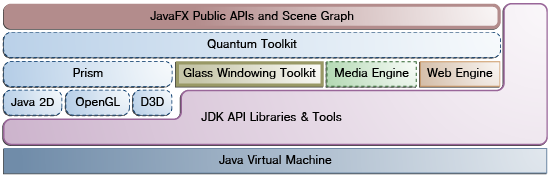
\includegraphics[scale=0.7]{Gambar/arsitekturJavaFX}
	\caption{Arsitektur JavaFX}
	\end{figure}
	
Ilustrasi dari gambar \textbf{2.1} mendeskripsikan setiap komponen saling berhubungan. Dibawah JavaFX Public API terdapat mesin yang menjalankan code JavaFX. Mesin tersebut terdiri dari sub komponen termasuk mesin grafis berperforma tinggi yang dinamakan Prism. Selain itu, terdapat sistem \textit{windowing} kecil dan efisien yang dinamakan Glass. Terakhir dalam mesin dibawah JavaFX Public API terdapat sebuah \textit{media engine} dan \textit{web engine}. Berikut ini elemen-elemen yang terdapat pada arsitektur Java FX : \cite{javafx}
\begin{enumerate}
	\item \textit{Scene Graph}
	\item Java Public API untuk Fitur Java FX
	\item \textit{Graphics System}
	\item \textit{Glass Windowing Toolkit}
	\item Gambar dan Media
	\item Komponen Web
	\item CSS
	\item \textit{UI Control}
	\item Layout
	\item Transformasi 2-D dan 3-D
	\item \textit{Visual Effecs}
\end{enumerate}

\subsection{Scene Graph}
\textit{Scene Graph} merupakan sebuah pohon hirarki dari sekumpulan node yang merepresentasikan elemen visual dari antarmuka suatu aplikasi. Sebuah elemen dari \textit{scene graph} dinamakan node. Setiap node mempunya ID, \textit{style class} dan \textit{boundling volume}. Node dalam \textit{scene graph} juga memiliki :\cite{javafx}
\begin{enumerate}
	\item \textit{Effect}, seperti blur dan shadow
	\item \textit{Opacity}
	\item \textit{Transform}
	\item \textit{Event handler} (Mouse, keyboard, dan input method lainnya)
	\item Perintah spesifik dari sebuah aplikasi
\end{enumerate} 

Penggunaan \textbf{javafx.scene} API memungkinkan \textit{developer} untuk menggunakan beberapa jenis konten dialamnya, seperti : \cite{javafx}
\begin{enumerate}
	\item \textbf{Node} : Bentuk(2-D dan 3-D), gambar, media, \textit{embedded web browser}, teks, \textit{UI control}, grafik, grup, dan \textit{container}.
	\item \textbf{State} : Transformasi (posisi dan orientasi dari node), efek visual, dan konten visual lainnya.
	\item \textbf{Effect} : objek sederhana yang dapat merubah penampilan dari node \textit{scene graph}, seperti blur, shadow, dan \textit{color adjustment}
\end{enumerate}

\subsection{Java Public API untuk Fitur Java FX}
Pada lapisan atas arsitektur Java FX pada gambar \textbf{2.1} API Java memberikan kebebasan dan fleksibilitas untuk membangun berbagai client dari sebuah aplikasi. Platform Java FX menggabungkan kemampuan terbaik yang dimiliki platform Java secara menyeluruh dan mendalam serta intuitif dengan memasukan fungsi media kedalamnya, sehingga tercipta lingkup konsep \textit{one-stop development}. Berikut contoh kegunaan Java API untuk fitur Java FX :\cite{javafx}
\begin{enumerate}
	\item Memungkinkan penggunaan fitur Java yang poweful seperti \textit{generics, annotations, multithreading}.
	\item Lebih mudah mengembangan web menggunakan Java FX dibanding \textit{JVM-base dynamic languages} lainnya seperti Grovvy, dan JavaScript.
	\item Memungkinkan Java developer untuk menggunakan bahasa sistem seperti Groovy untuk menulis file besar atau kompleks pada aplikasi Java FX.
	\item Memungkinkan penggunaan binding.
	\item Menambahkan koleksi library Java dengan memasukan urutan dan memetakan perubahan sehingga memngukinkan aplikasi untuk menghubungkan antarmuka kedalam data model, mengamati perubahan pada data model, dan memperbarui kontrol UI yang sesuai dengan perubahan tersebut.   
\end{enumerate}

\subsection{Graphic System}
\textit{Java FX Graphic System} pada gambar \textbf{2.1} merupakan implementasi dari Java FX \textit{scene graph layer}. Sistem grafis pada Java FX mendukung tampilan 2-D dan 3-D, selain itu sistem grafis ini menyediakan \textit{software rendering} untuk mendukung akselerasi \textit{rendering} dari \textit{hardware}. Berukut ini merupakan dua \textit{graphic accelerated pipeline} yang ada pada Java FX platform :\cite{javafx}
\begin{enumerate}
	\item \textbf{Prism} yang bekerja pada proses render. Prism dapat bekerja pada kedua sisi baik \textit{hardware} maupun \textit{software} rendering termasuk 3-D rendering. Prism juga bertanggung jawab untuk proses \textit{rasterization}(mengubah vektor menjadi pixel atau dot) dan rendering pada Java FX.
	\item \textbf{Quantum Toolkit} merupakan perpaduan Prism dan Windowing Toolkit yang bekerja di lapisan teratas pada Java FX untuk mengatur \textit{threading rule} yang berhubungan dengan rendering dan \textit{event handling}. 
\end{enumerate}

\subsection{Glass Windowing Toolkit}
Tugas pada lapisan ini adalah membantu \textit{service} pada sistem operasi, seperti mengatur windows, waktu , dan \textit{surface}. Glass Toolkit juga bertanggung jawab atas pengaturan \textit{event queue}.\cite{javafx}

\subsection{Media dan Gambar}
Fungsi -fungsi media pada Java FX tersedia pada \textbf{javafx.scene.media} API. Java FX mensuport baik visual maupun audio. Beberapa format yang disuport seperti MP3, AIFF, WAV pada file audio dan format FLV pada video. Ada tiga komponen yang berperan pada Java FX media, yaitu :\cite{javafx} 
\begin{itemize}
	\item \textit{Media object} merepresentasikan sebuah file media.
	\item \textit{Media Player} memutar sebuah file media.
	\item \textit{Media View} merupakan sebuah node yang menampilkan media tersebut.
\end{itemize}

\subsection{Komponen Web}
Mesin Web pada Java FX merupakan bagian dari Java FX UI control yang berbasis Webkit, dimana mesin web ini dapat menampilkan sebuah website dan melakukan browsing melalui APInya. Berikut ini fitur Java FX yang dapat di implementasikan pada program java :\cite{javafx}
\begin{enumerate}
	\item Render konten HTML dari local atau remote URL.
	\item Mendukung history dan menyediakan navigasi Back dan Forward.
	\item \textit{Reload Content}.
	\item Edit konten HTML.
	\item Mengeksekusi perintah JavaScript.
	\item \textit{Handle event}.
\end{enumerate} 

Komponen dari browser tersebut terbagi kedalam ke kelas-kelas berikut :\cite{javafx}
\begin{enumerate}
	\item \textbf{WebEngine} : menyediakan kemampuan dasar dari halaman web.
	\item \textbf{WebView} : merangkum sebuah \textit{WebEngine object}, Menggabungkan konten HTML kedalam layar aplikasi, dan mendukung \textit{field} dan \textit{method} untuk menerapkan efek dan transformasi berupa ekstensi maupun sebuah kelas Node.
\end{enumerate}

\subsection{CSS}
JavaFX Cascading Style Sheet (CSS) mendukung kemampuan untuk mengkustom styling pada antarmuka sebuah aplikasi Java FX tanpa merubah \textit{source code} aplikasi tersebut.\cite{javafx}   

\subsection{UI Control}
Java FX UI Control dalam Java FX API dibangun menggunakan node pada scene graph. Java FX UI Control dapat mengambil keuntungan dari fitur yang diberikan platform Java FX dan bersifat \textit{portable} pada platform yang berbeda.\cite{javafx}

\begin{figure}[H]
	\centering
	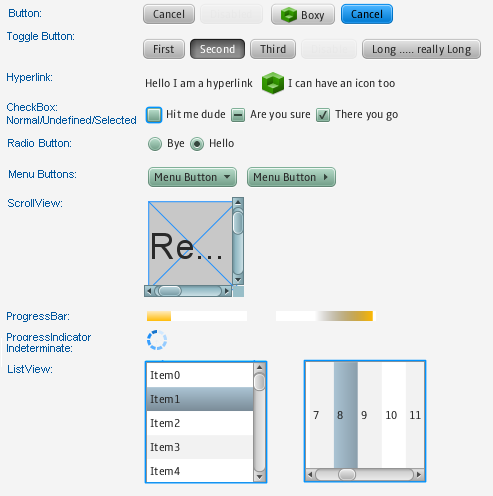
\includegraphics[scale=0.8]{Gambar/JavaFXuicontrols}
	\caption{Contoh Java FX UI Control}
	\end{figure}
	
	pada gambar \textbf{2.2} menunjukan UI Control yang sementara didukung oleh Java FX. Java UI control baru seperti TitlePane atau Accordion sebelumnya telah diperkenalkan pada Java FX SDK. UI control tersebut terdapat pada \textbf{javafx.scene.control} \textit{package}.\cite{javafx}
 
\subsection{Layout}
 \textit{Layout container} atau panel digunakan untuk pengatruan UI control secara dinamis dan fleksibel dalam scene graph pada aplikasi Java FX. Java FX Layout API mempunyai kelas-kelas yang dapat mengotomatiskan tata letak model sebagai berikut:\cite{javafx}
\begin{enumerate}
	\item \textbf{BorderPane} merupakan kelas yang mengatur bagian atas, bawah, kiri, kanan layout.
	\item \textbf{Hbox} merupakan kelas yang mengatur konten node secara horizontal dalam satu baris.
	\item  \textbf{Vbox} merupakan kelas yang mengatur konten node secara vertikal dalam satu baris.
	\item \textbf{StackPane} adalah kelas yang menempatkan \textit{back-to-front} konten node pada suatu \textit{stack}.
	\item \textbf{GridPane} adalah kelas yang memungkinkan developer untuk mebuat sebuah grid baris dan kolom secara flexible untuk memetakan konten node.
	\item \textbf{FlowPane} adalah kelas yang mengatur alur konten node baik horizontal maupun vertical, \textit{wrapping} pada batas lebar konten (untuk horizontal) atau tinggi konten (untuk vertical).
	\item \textbf{AnchorPane} adalah kelas yang memungkinkan developer untuk membuat \textit{anchor} node pada layout atas, bawah, sisi kiri atau ditengah layout. 
\end{enumerate}

\subsection{Transformasi 2-D dan 3-D}
Setiap node pada Java FX scene graph dapat ditransformasikan dalam koordinat x-y melalui kelas-kelas \textit{javafx.scene.transform} berikut ini:\cite{javafx}
\begin{enumerate}
	\item \textbf{translate} - Memindahkan sebuah node dari satu posisi ke posisi lain bersama koordinat x,y,z yang relatif terhadap posisi awalnya.
	\item \textbf{scale} - Meresize sebuah node untuk membesar atau mengecil sesuai koordinat x,y,z tergantung skala faktornya.
	\item \textbf{rotate} - Merotasi sebuah node sesuai titik porosnya.
	\item \textbf{affine} - Melakukan pemetaan linear dari koordinat 2-D / 3-D ke koordinat 2-D / 3-D lainnya dengan menjaga lurus dan paralel sifat garis tersebut. Kelas ini digunakan bersamaan dengan kelas lainya dibanding penggunaan langsung.
\end{enumerate}

\subsection{Efek Visual}
Pengembahan antarmuka pada Java FX scene graph melibatkan \textit{Visual Effect} atau efek untuk meningkatkan tamoilan aplikasi Java FX secara \textit{real time}. Beberapa efek visual yang terdapat pada Java FX termasuk penggunaannya ada pada kelas - kelas berikut ini :\cite{javafx}
\begin{enumerate}
	\item \textbf{Drop Shadow} - Kelas ini merender sebuah bayangan dari konten yang ada dibelakang konten dimana efek tersebut diterapkan.
	\item \textbf{Reflection} - Kelas ini merender versi pantulan dari konten dibawah konten sebenarnya.
	\item \textbf{Lighting} - Kelas ini mensimulasikan sumber cahaya yang didapat dari konten dan memberikannya pada sebuah objek flat agar lebih nyata memberikan efek tiga dimensi.
\end{enumerate}

\subsection{Komponen Java FX}
Berikut ini merupakan kumpulan \textit{package} yang ada dalam Java FX\cite{javafx3}.\\
	\begin{tabular}{|c|p{12cm}|}
		\hline
		\textbf{No} & \textbf{Package dan Deskripsi} \\ \hline \hline
		1 & \textbf{javafx.application}\\
			&	Menyediakan kelas-kelas dalam siklus aplikasi.\\ \hline
		2 & \textbf{javafx.event}\\
			&	Memberikan kerangka dasar untuk FX event, dari mulai pengiriman hingga handling.\\ \hline	
		3 & \textbf{javafx.fxml}\\
			&	Berisi kelas untuk membuat hirarki objek dari markup.\\ \hline
		4 & \textbf{javafx.scene}\\
			&	Memberikan set basis kelas - kelas untuk Java FX Scene Graph API .\\ \hline
		5 & \textbf{javafx.scene.control}\\
			&	Java FX \textit{User Interface Control }(kontrol UI atau kontrol saja) dimana node khusus dalam Java FX Scenegraph yang dapak digunakan untuk banuak konteks aplikasi yang berbeda.\\ \hline
		6 & \textbf{javafx.scene.input}\\
			&	Menyediakan set kelas - kelas untuk mouse dan keyboard \textit{input event handling}.\\ \hline
		7 & \textbf{javafx.scene.input}\\
			&	Menyediakan set kelas - kelas untuk mouse dan keyboard \textit{input event handling}.\\ \hline
		8 & \textbf{javafx.scene.layout}\\
			&	Menyediakan kelas - kelas untuk mendukung UI layout.\\ \hline
		9 & \textbf{javafx.scene.text}\\
			&	Menyediakan set kelas - kelas untuk font dan teks node yang dapat di render.\\ \hline
		10 & \textbf{javafx.util}\\
			&	Berisi berbagai utilitas dan kelas pembantu.\\ \hline
		11 & \textbf{javafx.util.converter}\\
			&	\textit{Package} ini untuk konversi String pada Java FX.\\ \hline
		12 & \textbf{javafx.beans}\\
			&	\textit{Package} ini berisi interface yang mendefinisikan bentuk umum dari \textit{observability}.\\ \hline
		13 & \textbf{javafx.beans.binding}\\
			&	\textit{Package} ini untuk menjelaskan karakter dari \textit{Binding}.\\ \hline	
		14 & \textbf{javafx.beans.binding}\\
			&	\textit{Package} ini mendefinisikan \textit{read-only} properti dan \textit{writable} properti, ditambah sejumlah implementasi.\\ \hline		
	\end{tabular}

\subsection{javafx.application}
\textbf{}